\section{Data Quality} \label{sec:res_DataQuality}

%Initial hardware implementation show the accuracy of data from the eye tracker in question. A series of simple gaze fixation tests revealed the accuracy and noise inherent in the data produced, as well as the range of possible values full screen on a 24" 1920x1200 monitor. Data range was aquired by fixating on all four corners of the monitor. Accuracy and noise levels were measured in a steady, uninterrupted stream of gaze data where the user continually stared at a fixed point on screen for ten seconds. Test results are summarized in table \_.

Results presented will aim to paint a picture of the quality of data produced by the eye tracker detailed in section \ref{sec:hwds_TobiiEyeTracker5}. All results in this section were generated on a 24" 1920x1200 Dell monitor.

\subsection{Qualification Tests}

Results from the first qualification test conducted are presented in figure \ref{fig:res_GazePointTest} and aim to provide a general overview of data quality. Results were generated by instructing the subject to fixate on nine different points for three seconds each. These nine points were chosen to observe how gaze is output at differing degrees of visual angle, as well as edge cases. The farthest points were at the four very edges of the monitor. One was at the center and the rest on the diagonals in between. Around 100 samples were collected for each gaze point. The test was subsequently repeated three times in a controlled environment. That is, with unchanged device calibration while disallowing the subject to move in the tracking space.

\begin{figure}[h]
    \centering
    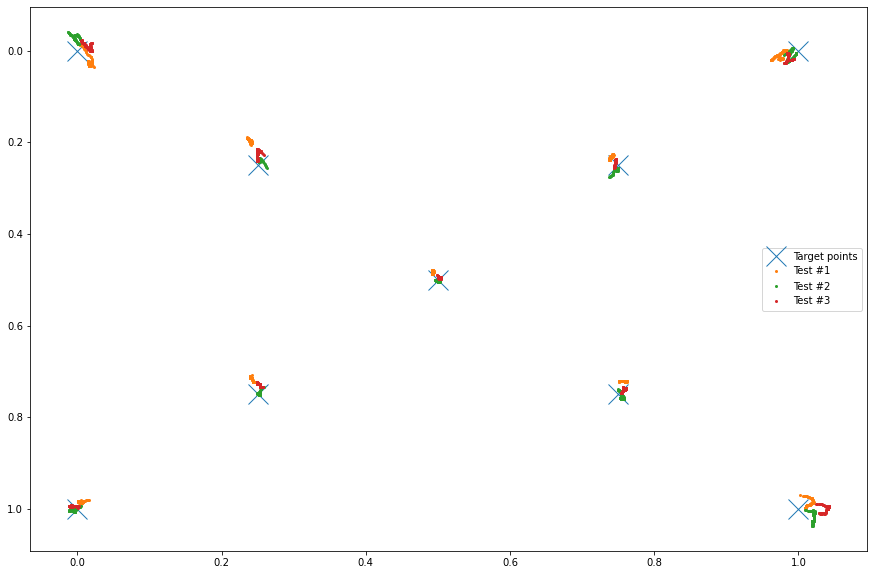
\includegraphics[width=0.8\textwidth]{Images/DataQuality/GazePointTest.png}
    \caption{Gaze point test results. The x- and y-axes represent on-screen coordinates, as they are output from Tobii ET5. The blue crosses are the gaze points on which the user was instructed to fix their gaze. Orange, green, and red dots represent single-sample representations of user gaze in the first, second, and third tests, respectively.}
    \label{fig:res_GazePointTest}
\end{figure}


Another qualification test was conducted to see whether scan paths produced by Tobii ET5 were consistent. Results are presented in figure \ref{fig:res_ScanpathTest}. This time, the subject was instructed to follow a moving target, traveling smoothly along all four borders of the monitor and along both diagonals. Again, the test was repeated three times. Each test lasted about 30 seconds, and around 3000 samples were collected in all.

\begin{figure}[h]
    \centering
    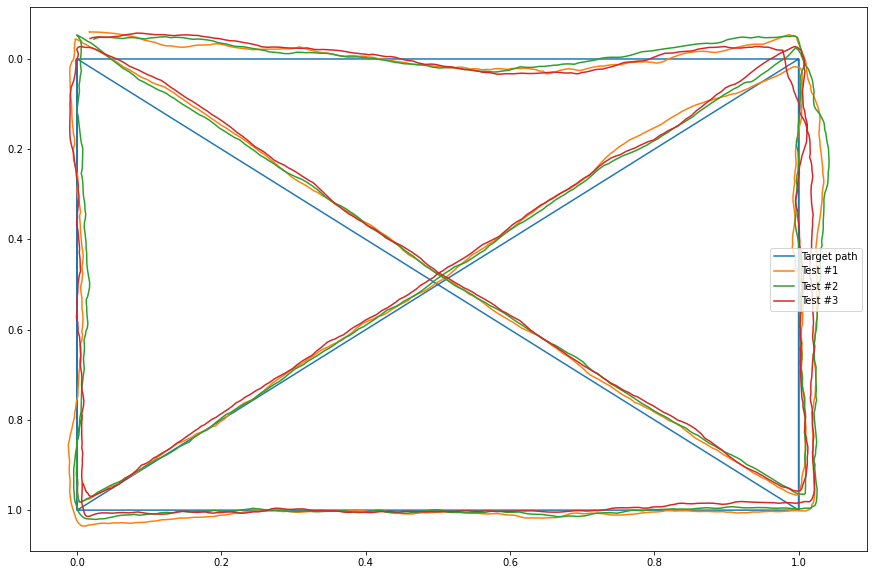
\includegraphics[width=0.8\textwidth]{Images/DataQuality/ScanpathTest.png}
    \caption{Scan path test results. Once again, the x- and y-axes represent on-screen coordinates, as they are output from Tobii ET5. The straight blue lines are the target paths which the user was instructed to follow with their gaze. }
    \label{fig:res_ScanpathTest}
\end{figure}

Figure \ref{fig:res_PaperHeatmap} attempts to illustrate a possible application of eye-tracking data with one final test. Here, the subject was instructed to read one page of a paper and terminate the recording once the task was complete. In the end, a heatmap was generated from the data. Both heatmap and paper are presented here. 
%As we can see, the eye tracker has an accuracy which allows for clear distinctions of paragraphs and lines.

\begin{figure}
    \centering
    \begin{minipage}{0.5\textwidth}
        \centering
        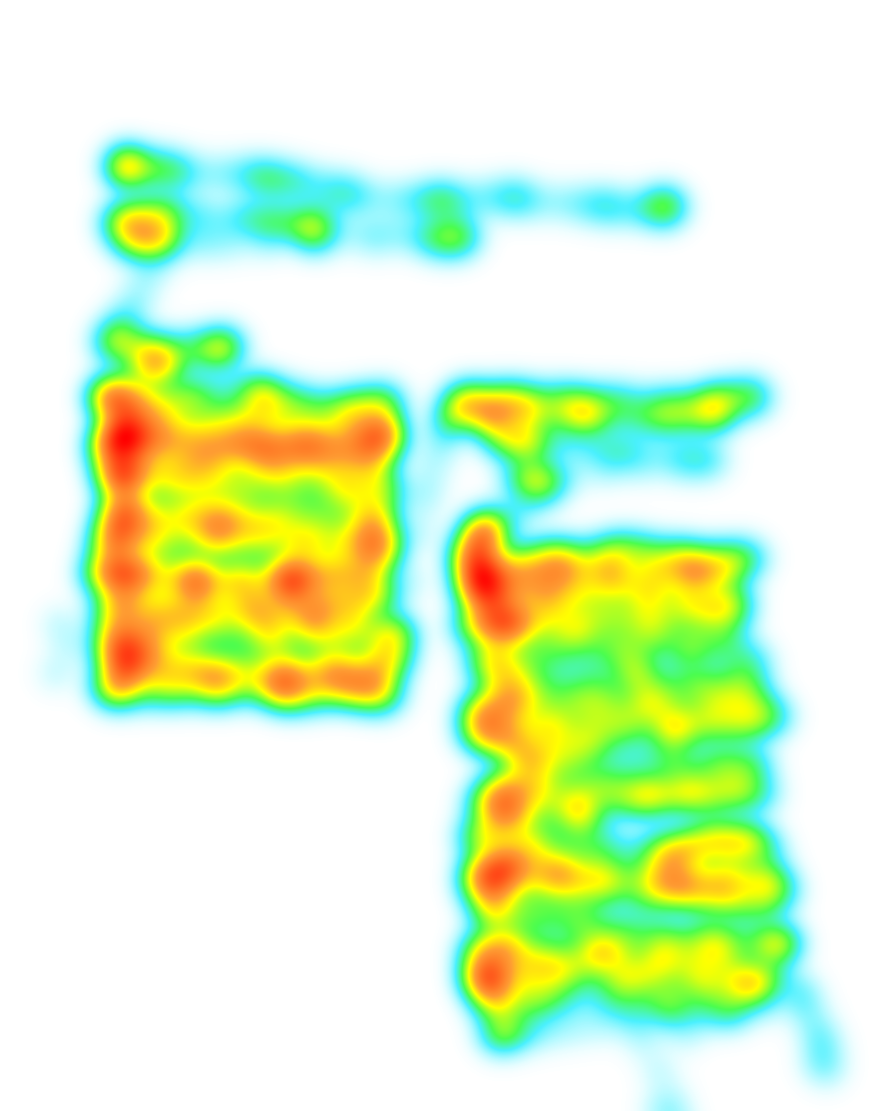
\includegraphics[width=0.8\textwidth]{Images/DataQuality/PaperHeatmap.png}
        %\caption{first figure}
    \end{minipage}\hfill
    \begin{minipage}{0.5\textwidth}
        \centering
        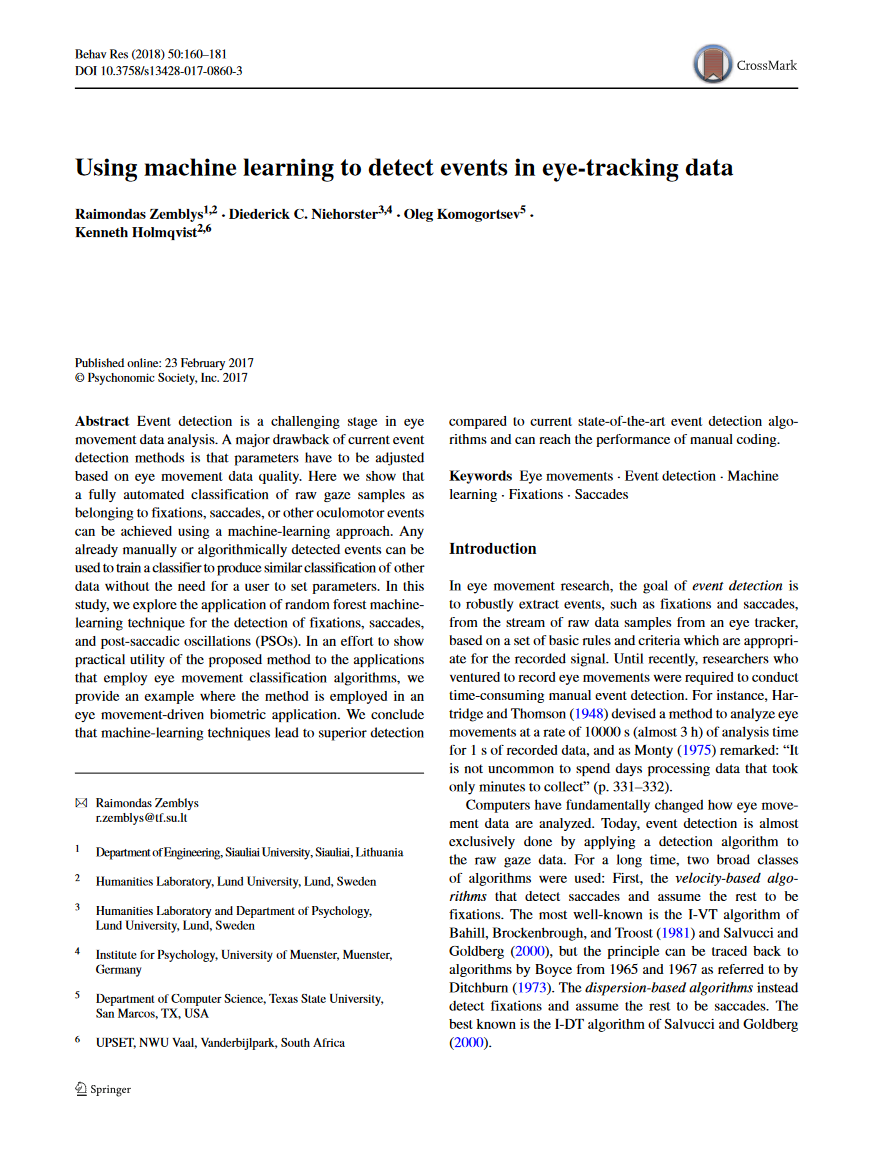
\includegraphics[width=0.8\textwidth]{Images/DataQuality/Paper.png}
        %\caption{second figure}
    \end{minipage}
    \caption{Heat map test. Color gradient from cyan to red indicate fixation duration from brief to long. The right figure shows the paper that was read.}
    \label{fig:res_PaperHeatmap}
\end{figure}

\subsection{Other Insights}

To gain concrete insight into the fundamental statistical properties of the data stream, I present figure \ref{fig:res_DataDeviations}. These violin plots were all generated on the data gathered during the first repetition of the gaze point test of figure \ref{fig:res_GazePointTest}. Each violin of each plot represents the deviations in on-screen coordinates of one sample on one axis from the mean of one observed set of data samples. Since the mean values of each point are subtracted from each violin, these plots do not account for bias. Each of these sets of data samples comes from the user fixating at one of the nine gaze points of figure \ref{fig:res_GazePointTest}. Plots in the same column are generated from the same target gaze point groups. Groups are organized in edge, diagonal, and center points. The top row of plots shows deviations in the y-coordinate axis, while the bottom row shows the same on the x-axis.

\begin{figure}[h]
    \centering
    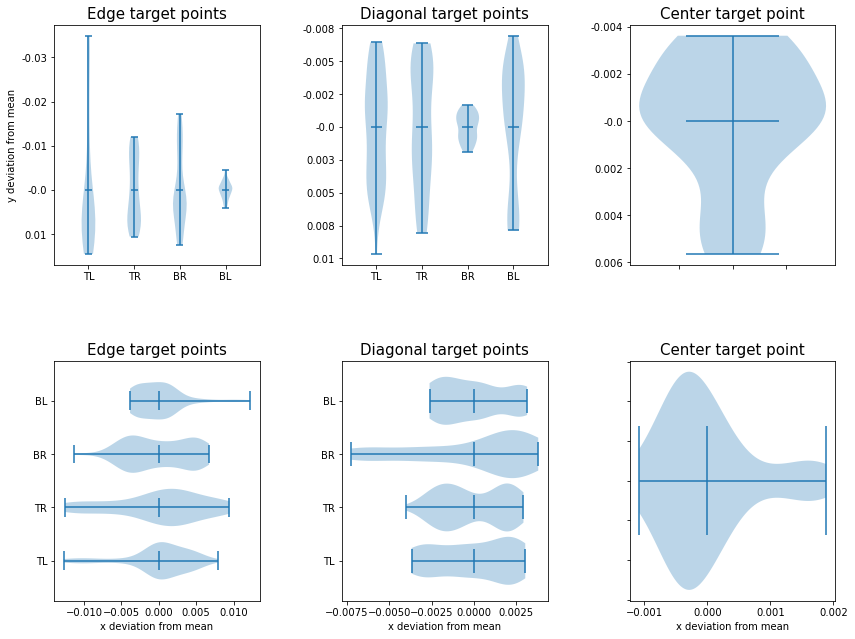
\includegraphics[width=0.8\textwidth]{Images/DataQuality/DataDeviations.png}
    \caption{Data deviations. Columns share target gaze point types, rows share coordinate axes. For edge- and diagonal target plots, each violin represent either the top-left (TL), top-right (TR), bottom-right (BR), or bottom-left (BL) gaze target points. Note that the coordinate axes are scaled to match the values of each plot.}
    \label{fig:res_DataDeviations}
\end{figure}

Accompanying figure \ref{fig:res_DataDeviations} is table \ref{tab:res_DataStats}, which illustrates typical occurrences of bias and variance in the data output. As with figure \ref{fig:res_DataDeviations}, this data was gathered from the first iteration of the gaze point test, representing related information. Additionally, bias is inferred by individually calculating the median position on both coordinate axes and subtracting the target point coordinates.

\import{./}{DataTable}

Finally, the effects of data drift are given in figure \ref{fig:res_DataDeviations}. This plot is taken from all repetitions of the gaze point test of figure \ref{fig:res_GazePointTest} and is merely centered on and scaled up to only show the fine-grained evolution of gaze points during fixation. This particular point is at the top-left corner of the monitor. 

\begin{figure}[h]
    \centering
    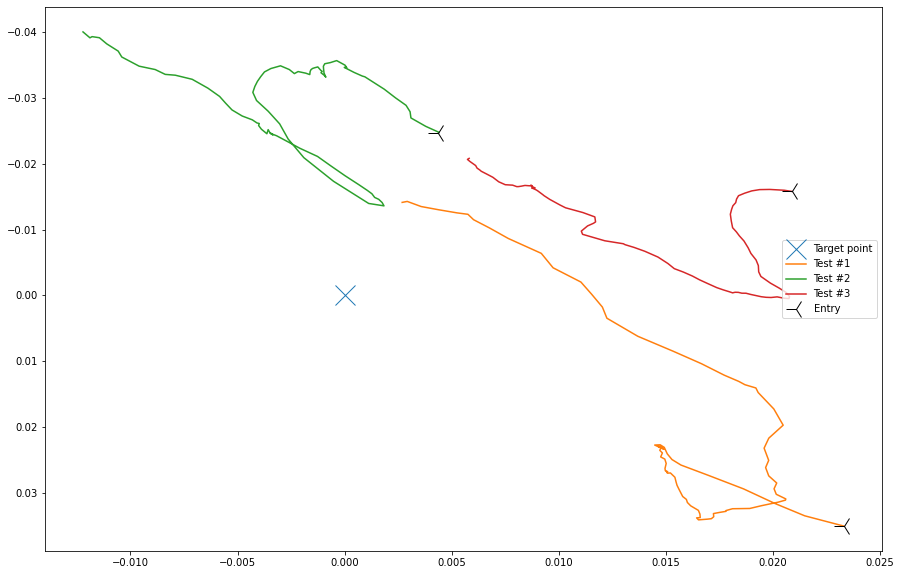
\includegraphics[width=0.8\textwidth]{Images/DataQuality/DataDrift.png}
    \caption{Effects of data drift. Again, the x- and y-axes represent on-screen coordinates, as they are output from Tobii ET5. The single blue cross is the top-left target gaze point observable in figure \ref{fig:res_GazePointTest}. Orange, green, and red lines show the between-sample scan paths of user gaze in the first, second, and third tests, respectively. The black tri-crosses are the entry points from which the scan path evolves.}
    \label{fig:res_DataDrift}
\end{figure}



